\documentclass[11pt]{article}

\usepackage[T1]{fontenc}
\usepackage[utf8]{inputenc}
\usepackage[spanish,provide=*]{babel}
\usepackage{mathpazo}
\usepackage[scaled=0.92]{helvet}
\usepackage{microtype}
\usepackage[margin=2.6cm]{geometry}
\usepackage{amsmath,amssymb,amsthm}
\usepackage{bm}
\usepackage{booktabs}
\usepackage{tabularx}
\usepackage{longtable}
\usepackage{multirow}
\usepackage{graphicx}
\usepackage{caption}
\usepackage{enumitem}
\usepackage{xcolor}
\usepackage{tikz}
\usetikzlibrary{arrows.meta,positioning,calc,fit,backgrounds,shapes.geometric}
\usepackage{pgfplots}
\pgfplotsset{compat=1.18}
\usepackage{algorithm}
\usepackage{algpseudocode}
\usepackage[round,authoryear]{natbib}
\usepackage[colorlinks=true,linkcolor=blue!50!black,citecolor=blue!50!black,urlcolor=blue!50!black]{hyperref}

\captionsetup{font=small,labelfont=bf}
\urlstyle{same}
\setlist{itemsep=2pt,topsep=4pt}

\newtheorem{proposicion}{Proposición}
\newtheorem{lema}{Lema}
\theoremstyle{definition}
\newtheorem{definicion}{Definición}
\newtheorem{invariante}{Invariante}
\theoremstyle{remark}
\newtheorem{observacion}{Observación}
\newtheorem{ejemplo}{Ejemplo}

\floatname{algorithm}{Algoritmo}
\algrenewcommand\algorithmicrequire{\textbf{Entrada:}}
\algrenewcommand\algorithmicensure{\textbf{Salida:}}

\newcommand{\Pre}{\operatorname{Pre}}
\newcommand{\Post}{\operatorname{Post}}
\newcommand{\Rh}{\hat R}
\newcommand{\Sh}{\hat S}
\newcommand{\Lh}{\hat L}
\newcommand{\Pih}{\hat\Pi}
\newcommand{\rstar}{r^{\ast}}
\newcommand{\Slisto}{S_{\mathrm{listo}}}
\newcommand{\Smin}{S_{\min}}
\newcommand{\Hist}{\mathcal H}
\newcommand{\Dom}{\mathcal D}
\newcommand{\Banco}{\mathcal B}
\newcommand{\Carga}{\mathcal L}

\definecolor{azul}{HTML}{2A78D6}
\definecolor{naranja}{HTML}{EB6834}
\definecolor{verde}{HTML}{1B8F66}
\definecolor{gris}{HTML}{52514E}
\definecolor{morado}{HTML}{6250D6}

\title{\textbf{Arquitectura conceptual de un sistema de repetición espaciada para habilidades procedimentales}\\[4pt]
\large Ecuaciones, supuestos y componentes, con aplicación a la física clásica de preparatoria}
\author{Gustavo S. de la Rosa\\[2pt]\small Proyecto de maestría --- documento técnico, segunda versión}
\date{Noviembre de 2026}

\begin{document}
\maketitle

\begin{abstract}
\noindent Este documento describe a detalle el modelo y la arquitectura del sistema de repetición espaciada para habilidades procedimentales que proponemos en el proyecto de maestría. A diferencia del primer artículo, que se centró en la evaluación por simulación, aquí el objetivo es explicar \emph{qué calcula cada ecuación, de dónde sale y qué supuestos introduce}, y describir la \emph{arquitectura conceptual} del sistema: qué componentes lo forman, qué información intercambian, qué invariantes deben cumplir y en qué escalas de tiempo operan, sin depender de ninguna tecnología de implementación. Por ahora el sistema se limita a la física clásica (mecánica) de preparatoria: un grafo de 15 unidades y 168 subtemas, del que un prototipo usa un subgrafo de 13 subtemas de cinemática. El modelo combina el olvido exponencial y la dinámica de saltos de \citet{tabibian2019} con una matriz $Q$ fraccional, un modelo de observación conjuntivo con descuido y adivinanza, una asignación bayesiana de culpa, una regla de admisión con control de carga y un planificador por cobertura submodular. Incluimos las derivaciones de cada ecuación, un ejemplo numérico de punta a punta, un resumen de la evidencia de simulación y la correspondencia entre la arquitectura abstracta y el prototipo construido.
\end{abstract}

\tableofcontents
\bigskip

%=====================================================================
\section{Introducción}
%=====================================================================

Los sistemas de repetición espaciada deciden \emph{cuándo} volver a practicar algo para que no se olvide. Funcionan muy bien con hechos aislados (vocabulario, fechas, definiciones), donde cada tarjeta ejercita una sola pieza de conocimiento y las tarjetas son independientes entre sí. Resolver un problema de física es distinto. Un problema de tiro parabólico exige descomponer un vector, aplicar las ecuaciones del movimiento acelerado y combinar los movimientos horizontal y vertical. Si el estudiante falla, no sabemos cuál de esas piezas falló. Y existe un orden natural de aprendizaje: sin movimiento acelerado no hay tiro parabólico.

El proyecto busca un sistema que conserve la idea central de la repetición espaciada (repasar justo cuando el recuerdo empieza a debilitarse) y la extienda a \emph{habilidades repetibles}: procedimientos que se ejecutan una y otra vez sobre datos distintos. El primer documento del proyecto presentó el modelo y lo evaluó con un simulador. Este segundo documento tiene dos propósitos:

\begin{enumerate}
\item \textbf{Explicar las ecuaciones con detalle} (\S\ref{sec:ecuaciones}): para cada una, qué calcula, de dónde sale, qué significan sus parámetros, cómo se comporta en los casos límite y un ejemplo con números.
\item \textbf{Describir la arquitectura conceptual} (\S\ref{sec:arquitectura}): los componentes del sistema y sus relaciones, descritos como objetos matemáticos y flujos de información, de modo que el diseño sea independiente de si se implementa como aplicación web, aplicación móvil, servidor o incluso a mano en una hoja de cálculo.
\end{enumerate}

\paragraph{Alcance.} Por ahora el sistema trata \textbf{únicamente la física clásica de preparatoria}, en particular la mecánica (\S\ref{sec:dominio}). No cubre otras áreas de la física (termodinámica, ondas, electromagnetismo) ni matemáticas, aunque la arquitectura está pensada para que extenderlo sea cambiar el \emph{contenido} (el grafo y el banco de problemas) sin cambiar el \emph{modelo}.

%=====================================================================
\section{El dominio: física clásica de preparatoria}
\label{sec:dominio}
%=====================================================================

\subsection{El temario como grafo}

El dominio se describe con un grafo dirigido acíclico en el que una flecha $A\to B$ significa que $A$ es prerrequisito de $B$. La Figura~\ref{fig:grafo-fisica} muestra el temario de mecánica de preparatoria organizado en 15 unidades y 7 áreas temáticas: bases matemáticas y herramientas, cinemática, dinámica, cantidad de movimiento e impulso, trabajo y energía, sistemas, y temas de cierre.

\begin{figure}[t]
\centering
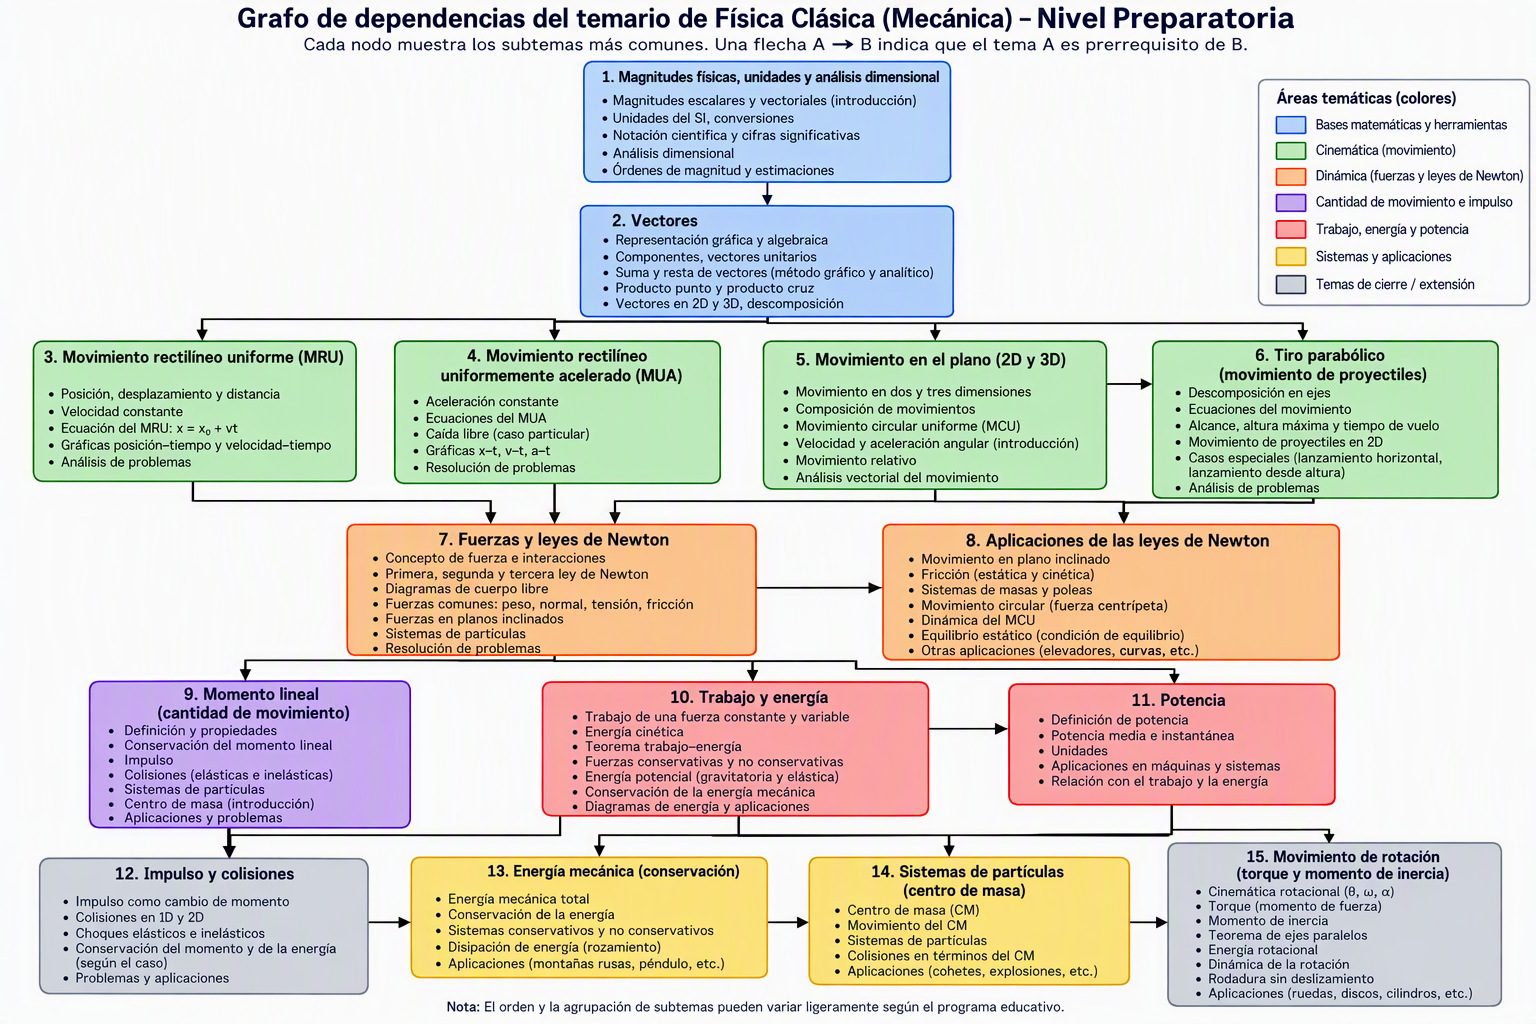
\includegraphics[width=\textwidth]{figuras/grafo_fisica.png}
\caption{Grafo de dependencias del temario de física clásica (mecánica) de nivel preparatoria. Cada nodo es una unidad con sus subtemas más comunes; una flecha $A\to B$ indica que $A$ es prerrequisito de $B$.}
\label{fig:grafo-fisica}
\end{figure}

La figura es la representación visual del temario. La especificación formal que usan el simulador y el prototipo es una lista de 26 aristas entre unidades (Apéndice~\ref{app:aristas}). Hay que reconciliar ambas: algunas flechas parecen estar en la figura y no en la lista (por ejemplo MRU $\to$ Leyes de Newton, Impulso $\to$ Energía mecánica y Energía mecánica $\to$ Sistemas de partículas). Mientras tanto, cuando difieran, manda la lista.

\subsection{Granularidad: unidades, subtemas y habilidades}

El modelo trata cada nodo del grafo como \emph{una habilidad con una sola memoria}. Por eso importa la granularidad:

\begin{itemize}
\item \textbf{Unidades} (15 nodos). Demasiado gruesas: ``Aplicaciones de las leyes de Newton'' agrupa planos inclinados, poleas y curvas peraltadas, que no se olvidan en bloque. En simulación, a este nivel el sistema propuesto no supera a un Anki SM-2 bien configurado.
\item \textbf{Subtemas} (168 nodos, 279 dependencias, 21 niveles de profundidad). Es el nivel que usamos. Cada subtema es un procedimiento identificable (``alcance horizontal'', ``fuerza de fricción cinética'') para el que se pueden escribir problemas paramétricos. Las dependencias se anotaron a mano a nivel de subtema y están pendientes de validación docente.
\item \textbf{Prototipo} (13 subtemas). Un subgrafo de cinemática, de conversión de unidades a alcance horizontal (Apéndice~\ref{app:prototipo}), con 33 plantillas de problemas.
\end{itemize}

\subsection{Por qué la física de preparatoria es un buen primer dominio}

\begin{enumerate}
\item \textbf{Procedimientos explícitos.} Casi todo problema se resuelve aplicando procedimientos nombrables (descomponer, despejar, sustituir), lo que facilita definir habilidades.
\item \textbf{Prerrequisitos claros.} El orden del temario es estable entre programas educativos.
\item \textbf{Problemas paramétricos.} Un mismo problema admite infinitas instancias cambiando los datos. Así se evita que el estudiante memorice respuestas en lugar de ejecutar el procedimiento.
\item \textbf{Respuestas verificables.} La mayoría de las respuestas son números con unidades, que se pueden calificar automáticamente con una tolerancia.
\end{enumerate}

\paragraph{Fuera del alcance actual:} explicaciones conceptuales abiertas, detección de concepciones erróneas específicas, problemas de varios pasos con calificación parcial, otras áreas de la física y las matemáticas. Las matemáticas son la extensión natural siguiente.

%=====================================================================
\section{Arquitectura conceptual}
\label{sec:arquitectura}
%=====================================================================

Describimos el sistema como un conjunto de objetos matemáticos y funciones entre ellos. La descripción no supone lenguaje, base de datos ni plataforma; cualquier implementación que respete las firmas y los invariantes de esta sección es una instancia válida del diseño.

\subsection{Principio de separación}

La arquitectura separa cinco tipos de información que cambian por razones distintas y a ritmos distintos:

\begin{enumerate}
\item \textbf{Conocimiento del dominio} $\Dom$: qué hay que aprender y cómo se relaciona. Lo editan docentes; cambia por semestres.
\item \textbf{Parámetros del modelo} $\bm\theta$: cómo aprenden y olvidan los estudiantes \emph{en general}. Se estiman con datos; cambian cada que se recalibra.
\item \textbf{Parámetros de la política} $\bm\varphi$: decisiones pedagógicas (cuánto practicar por día, qué retención perseguir). Las fija el diseñador.
\item \textbf{Estado del estudiante} $\sigma$: lo que el sistema cree de \emph{este} estudiante. Cambia en cada intento.
\item \textbf{Historial} $\Hist$: lo que efectivamente ocurrió. Sólo crece.
\end{enumerate}

La separación más importante es la última: \emph{el historial es la fuente de verdad y el estado es una consecuencia}. El estado se puede reconstruir en cualquier momento repasando el historial con los parámetros vigentes (Invariante~\ref{inv:replay}). Eso permite recalibrar $\bm\theta$ sin perder nada y auditar cada decisión.

\subsection{Objetos}

\begin{definicion}[Dominio]
$\Dom=(G,W,\Banco)$, donde $G=(V,E)$ es un grafo dirigido acíclico de $K$ habilidades; $W=(w_{jk})\in[0,1]^{K\times K}$ es la matriz $Q$ fraccional (cuánto ejercita un problema del tipo $j$ a la habilidad $k$); y $\Banco=\{\tau\}$ es un banco de plantillas. Cada plantilla $\tau$ pertenece a una habilidad $h(\tau)$ y define una distribución sobre instancias $x$, cada una con un enunciado, una respuesta correcta $a(x)$, una tolerancia y una solución paso a paso.
\end{definicion}

\begin{definicion}[Estado del estudiante]
$\sigma=\{(\iota_k,\Sh_k,\Lh_k)\}_{k=1}^K$, donde $\iota_k\in\{0,1\}$ indica si la habilidad se ha introducido, $\Sh_k>0$ es su estabilidad estimada (en días) y $\Lh_k$ es el instante efectivo de su último repaso. El estado incluye además el conjunto $D_t$ de habilidades ya actualizadas en la sesión del día $t$.
\end{definicion}

\begin{definicion}[Parámetros]
Los del modelo y los de la política son, respectivamente,
\[
\bm\theta=(\Sh_0,G,\lambda,s,g,w_{\mathrm{pre}},\Smin),\qquad \bm\varphi=(\rstar,r_{\min},\Slisto,\rho,U,n_{\mathrm{intro}},m_{\max}).
\]
La Tabla~\ref{tab:parametros} los resume.
\end{definicion}

\begin{definicion}[Historial]
Una sucesión ordenada en el tiempo de eventos $\Hist=(e_1,e_2,\dots)$ de tres tipos:
\begin{itemize}
\item \emph{introducción} $(t,\textsf{intro},k)$: la habilidad $k$ se presentó con un ejemplo resuelto;
\item \emph{intento} $(t,\textsf{intento},j,x,y)$: se presentó la instancia $x$ de una plantilla de la habilidad $j$ y el resultado fue $y\in\{0,1\}$;
\item \emph{cambio de dominio o de parámetros}, con su contenido.
\end{itemize}
El paso del tiempo no es un evento: el estado depende de $t$ a través de las ecuaciones de olvido.
\end{definicion}

\subsection{Funciones}

El sistema se compone de siete funciones. Las primeras cuatro son el ``modelo'' y las otras tres lo rodean:

\begin{center}\small
\begin{tabularx}{\textwidth}{@{}l>{\raggedright\arraybackslash}p{4.4cm}X@{}}
\toprule
Función & Firma & Qué hace \\
\midrule
Recuerdo & $\Rh_k(\sigma,t)\in[0,1]$ & Probabilidad estimada de recuperar la habilidad $k$ en el instante $t$ (\S\ref{sec:memoria}). \\
Predicción & $\hat P(\sigma,j,t;\bm\theta)\in[0,1]$ & Probabilidad de resolver un problema del tipo $j$ (\S\ref{sec:observacion}). \\
Actualización & $\Phi(\sigma,e;\bm\theta)\mapsto\sigma'$ & Incorpora un evento al estado (\S\ref{sec:actualizacion}). \\
Planificación & $\Psi(\sigma,t;\Dom,\bm\theta,\bm\varphi)\mapsto A_t$ & Arma la secuencia de actividades del día (\S\ref{sec:admision}--\ref{sec:planificador}). \\
Generación & $\Gamma(\tau)\mapsto x$ & Produce una instancia nueva de una plantilla. \\
Calibración & $\Theta(\Hist)\mapsto\hat{\bm\theta}$ & Estima los parámetros del modelo con el historial (\S\ref{sec:estimacion}). \\
Evaluación & $\mathcal E(\Hist,\bm\theta)\mapsto$ métricas & Calibración de predicciones, cobertura, retención. \\
\bottomrule
\end{tabularx}
\end{center}

La Figura~\ref{fig:arquitectura} muestra cómo se conectan.

\begin{figure}[t]
\centering
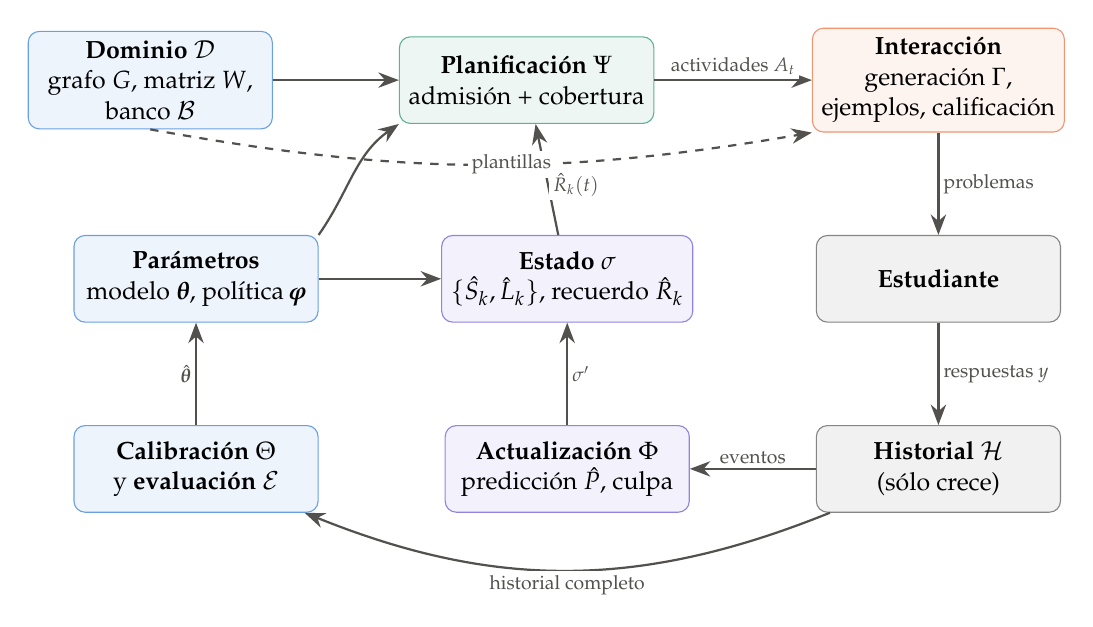
\begin{tikzpicture}[
  font=\small,
  caja/.style={draw=#1!70, fill=#1!8, rounded corners=4pt, minimum width=31mm, minimum height=11mm, align=center},
  fl/.style={-{Stealth[length=2.6mm]}, thick, gris},
  fll/.style={-{Stealth[length=2.6mm]}, thick, gris, dashed},
  lab/.style={font=\scriptsize, text=gris, fill=white, inner sep=1.5pt}
]
\node[caja=azul] (dom) {\textbf{Dominio} $\Dom$\\grafo $G$, matriz $W$,\\banco $\Banco$};
\node[caja=verde, right=16mm of dom] (plan) {\textbf{Planificación} $\Psi$\\admisión + cobertura};
\node[caja=naranja, right=20mm of plan] (int) {\textbf{Interacción}\\generación $\Gamma$,\\ejemplos, calificación};
\node[caja=gris, below=13mm of int] (est) {\textbf{Estudiante}};
\node[caja=gris, below=13mm of est] (hist) {\textbf{Historial} $\Hist$\\(sólo crece)};
\node[caja=morado, left=16mm of hist] (act) {\textbf{Actualización} $\Phi$\\predicción $\hat P$, culpa};
\node[caja=morado, above=13mm of act] (sigma) {\textbf{Estado} $\sigma$\\$\{\Sh_k,\Lh_k\}$, recuerdo $\Rh_k$};
\node[caja=azul, left=16mm of act] (cal) {\textbf{Calibración} $\Theta$\\y \textbf{evaluación} $\mathcal E$};
\node[caja=azul, above=13mm of cal] (theta) {\textbf{Parámetros}\\modelo $\bm\theta$, política $\bm\varphi$};

\draw[fl] (dom) -- (plan);
\draw[fl] (plan) -- node[lab, above]{actividades $A_t$} (int);
\draw[fl] (int) -- node[lab, right]{problemas} (est);
\draw[fl] (est) -- node[lab, right]{respuestas $y$} (hist);
\draw[fl] (hist) -- node[lab, above]{eventos} (act);
\draw[fl] (act) -- node[lab, right]{$\sigma'$} (sigma);
\draw[fl] (sigma) -- node[lab, right, pos=0.45]{$\Rh_k(t)$} (plan);
\draw[fl] (hist) to[bend left=22] node[lab, below]{historial completo} (cal);
\draw[fl] (cal) -- node[lab, left]{$\hat{\bm\theta}$} (theta);
\draw[fl] (theta) -- (sigma);
\draw[fl] (theta.north east) to[out=55, in=215] (plan.south west);
\draw[fll] (dom.south) to[bend right=10] node[lab, pos=0.55]{plantillas} (int.south west);
\end{tikzpicture}
\caption{Arquitectura conceptual. El ciclo de la derecha (planificación, interacción, historial, actualización) ocurre todos los días; el de la izquierda (calibración) ocurre cada que se acumulan datos suficientes. El estado $\sigma$ es una función del historial y de los parámetros.}
\label{fig:arquitectura}
\end{figure}

\subsection{Escalas de tiempo}

Las funciones operan en tres escalas:

\begin{center}\small
\begin{tabularx}{\textwidth}{@{}lXX@{}}
\toprule
Escala & Qué ocurre & Funciones \\
\midrule
Intento (segundos a minutos) & Se genera una instancia, el estudiante responde, se califica y se actualiza el estado. & $\Gamma$, $\hat P$, $\Phi$ \\
Sesión (un día) & El recuerdo de cada habilidad baja con el tiempo; se arma el plan del día. & $\Rh$, $\Psi$ \\
Ciclo lento (semanas o semestres) & Se recalibran los parámetros, se evalúa el modelo y se revisa el grafo. & $\Theta$, $\mathcal E$, edición de $\Dom$ \\
\bottomrule
\end{tabularx}
\end{center}

\subsection{Invariantes}

Cualquier implementación debe garantizar lo siguiente:

\begin{invariante}[El estado es una reproducción del historial]
\label{inv:replay}
Para todo $t$, $\sigma_t=\mathrm{Fold}(\Phi,\ \Hist_{\le t};\ \bm\theta)$: el estado se obtiene aplicando $\Phi$ a los eventos en orden. No hay información en $\sigma$ que no venga de $\Hist$ y $\bm\theta$.
\end{invariante}

\begin{invariante}[Una actualización por habilidad por sesión]
Si $k\in D_t$ (ya se actualizó hoy, o se introdujo hoy), ningún intento posterior del mismo día modifica $\Sh_k$.
\end{invariante}

\begin{invariante}[Respeto al grafo]
Una habilidad sólo se introduce si sus prerrequisitos cumplen la condición de admisión~\eqref{eq:admision}, y un problema sólo se presenta si sus componentes están introducidos.
\end{invariante}

\begin{invariante}[Carga acotada]
Al admitir habilidades nuevas, la carga esperada de mantenimiento más la de las nuevas no excede $\rho U$~\eqref{eq:carga-cond}.
\end{invariante}

\begin{invariante}[Instancias frescas]
Cada intento usa una instancia nueva $x=\Gamma(\tau)$, de una plantilla distinta de la última usada para esa habilidad cuando hay más de una. El estudiante no puede acertar recordando una respuesta.
\end{invariante}

\subsection{Puntos de extensión}

La separación hace que cada decisión de modelado viva en un solo lugar:

\begin{itemize}
\item \textbf{Otra curva de olvido} (ley de potencia, FSRS) sólo cambia $\Rh$ y la regla de acierto de $\Phi$; la planificación no se entera.
\item \textbf{Otro dominio} (matemáticas, química) sólo cambia $\Dom$.
\item \textbf{Otra pedagogía} (más práctica diaria, mayor retención objetivo) sólo cambia $\bm\varphi$.
\item \textbf{Modelos por estudiante} (efectos aleatorios) sólo cambian $\bm\theta$ y $\Theta$.
\end{itemize}

%=====================================================================
\section{Las ecuaciones, una por una}
\label{sec:ecuaciones}
%=====================================================================

\subsection{Notación}

\begin{center}\small
\begin{tabular}{@{}ll@{}}
\toprule
Símbolo & Significado \\
\midrule
$k,j$ & habilidades; $j$ suele ser el tema principal de un problema \\
$t$ & tiempo en días \\
$\Pre(k)$, $\Post(k)$ & prerrequisitos directos de $k$; habilidades que usan a $k$ directamente \\
$Q(j)=\{j\}\cup\Pre(j)$ & componentes de un problema del tipo $j$ \\
$w_{jk}$ & peso de la habilidad $k$ en un problema del tipo $j$ \\
$\Sh_k$, $\Lh_k$ & estabilidad estimada y último repaso efectivo de $k$ \\
$\Rh_k(t)$ & recuerdo estimado de $k$ en $t$ \\
$\Pih_j$, $\hat P_j$ & probabilidad de recuperar todos los componentes; de acertar el problema \\
$y\in\{0,1\}$ & resultado observado de un intento \\
$b_k$ & culpa de $k$ tras un fallo \\
$\Carga$ & carga esperada de mantenimiento \\
\bottomrule
\end{tabular}
\end{center}

\subsection{Matriz \texorpdfstring{$Q$}{Q} fraccional}

\begin{equation}
w_{jk}=\begin{cases}1 & k=j,\\ w_{\mathrm{pre}} & k\in\Pre(j),\\ 0 & \text{en otro caso.}\end{cases}
\label{eq:pesos}
\end{equation}

\paragraph{Qué calcula.} Cuánto ejercita un problema del tipo $j$ a cada habilidad. Un problema de caída libre ejercita por completo la caída libre ($w=1$) y a medias las ecuaciones del movimiento acelerado ($w=0.5$), que usa como herramienta.

\paragraph{Por qué fraccional.} En la psicometría clásica la matriz $Q$ es binaria \citep{tatsuoka1983}: el ítem requiere o no la habilidad. Un peso fraccional expresa que el prerrequisito se \emph{usa} sin ser el foco del problema. En el modelo, el peso aparece en tres lugares: como exponente en la probabilidad de recuperarlo~\eqref{eq:observacion}, como factor en la ganancia por acierto~\eqref{eq:acierto} y como fracción del salto~\eqref{eq:salto}.

\paragraph{Casos límite.} Con $w_{\mathrm{pre}}=0$ el modelo ignora los prerrequisitos (cada problema ejercita sólo su tema, como las tarjetas de Anki). Con $w_{\mathrm{pre}}=1$, practicar caída libre contaría igual que practicar movimiento acelerado. El valor $0.5$ es un supuesto; con datos se puede estimar un $w_{jk}$ por par.

\subsection{Memoria: olvido exponencial}
\label{sec:memoria}

\begin{equation}
\Rh_k(t)=\exp\!\left(-\frac{t-\Lh_k}{\Sh_k}\right)=e^{-\hat n_k\,\Delta t},\qquad \hat n_k=\frac1{\Sh_k},\qquad \Delta t=t-\Lh_k.
\label{eq:memoria}
\end{equation}

\paragraph{De dónde sale.} Es la solución de suponer que el recuerdo se pierde a una \emph{tasa proporcional a lo que queda}:
\[
\frac{d\Rh}{dt}=-\hat n\,\Rh,\qquad \Rh(\Lh)=1\quad\Longrightarrow\quad \Rh(t)=e^{-\hat n(t-\Lh)}.
\]
Es la curva de olvido de \citet{tabibian2019} y de la regresión de vida media de \citet{settles2016}. La tasa de olvido $\hat n$ es la variable natural en Tabibian; nosotros usamos su inversa, $\Sh=1/\hat n$, porque se lee en días.

\paragraph{Cómo leer $\Sh$.} $\Sh$ es el tiempo en que el recuerdo cae a $e^{-1}\approx0.37$. Hay otras lecturas útiles:
\begin{itemize}
\item cae a 90\% en $\Sh\ln(1/0.9)\approx0.105\,\Sh$ días;
\item cae a la mitad en $\Sh\ln2\approx0.69\,\Sh$ días;
\item cae a la retención objetivo $\rstar$ en $\Sh\ln(1/\rstar)$ días; con $\rstar=0.7$, en $0.357\,\Sh$.
\end{itemize}
Con $\Sh_0=8.2$, un tema recién introducido vence a los $2.9$ días.

\paragraph{Supuestos.} La forma exponencial supone que la tasa de olvido es constante entre repasos. La evidencia sugiere que el olvido real decae más lento en la cola (ley de potencia). Por eso en el simulador la ``verdad'' usa ley de potencia, y la calibración del modelo exponencial frente a esa verdad mide el costo del supuesto.

\paragraph{Por qué $\Lh_k$ y no ``la fecha del último repaso''.} Tras un repaso parcial (un prerrequisito con $w<1$) el recuerdo no vuelve a 1. Elegimos $\Lh_k$ como el instante \emph{ficticio} en el que, con la estabilidad actual, el recuerdo habría sido 1, de modo que la fórmula~\eqref{eq:memoria} siga valiendo (ver~\eqref{eq:salto}).

\subsection{Modelo de observación}
\label{sec:observacion}

\begin{equation}
\Pih_j(t)=\prod_{k\in Q(j)}\Rh_k(t)^{\,w_{jk}},\qquad
\hat P_j(t)=(1-s)\,\Pih_j(t)+g\,\bigl(1-\Pih_j(t)\bigr).
\label{eq:observacion}
\end{equation}

\paragraph{De dónde sale.} Suponemos que resolver el problema requiere recuperar \emph{todos} sus componentes (modelo \emph{conjuntivo}, como DINA; \citealp{junker2001}) y que las recuperaciones son independientes. Si el componente $k$ se recupera con probabilidad $\Rh_k^{\,w_{jk}}$, la probabilidad de recuperarlos todos es el producto $\Pih_j$. Después intervienen dos errores de observación:
\[
\Pr(y=1)=\underbrace{\Pr(\text{recupera todo})\,(1-s)}_{\text{sabe y no se descuida}}+\underbrace{\Pr(\text{no recupera algo})\,g}_{\text{no sabe pero acierta}}.
\]

\paragraph{Descuido $s$ y adivinanza $g$.} Vienen del rastreo bayesiano del conocimiento \citep{corbett1994}. $s=0.05$ representa errores aritméticos o de transcripción. $g=0.02$ es bajo porque los problemas son abiertos (hay que llegar a un número); en opción múltiple con cuatro opciones sería cercano a $0.25$. Con estos valores, $\hat P\in[g,\,1-s]=[0.02,\,0.95]$: el modelo nunca está seguro, y ningún resultado tiene probabilidad cero en la verosimilitud.

\paragraph{Por qué el peso va en el exponente.} Porque $\Rh^{\,w}=\exp(-w\,\Delta t/\Sh)$: un componente con peso $w$ se comporta como si hubiera estado expuesto al olvido sólo una fracción $w$ del tiempo. Un prerrequisito a medio olvidar estorba menos que el tema principal a medio olvidar. Por ejemplo, con $\Rh=0.6$, la probabilidad de recuperarlo es $0.6$ si es el tema principal y $0.6^{0.5}=0.77$ si es un prerrequisito.

\paragraph{Supuesto de independencia.} Las recuperaciones de los componentes probablemente están correlacionadas (un estudiante distraído falla todo). El efecto es que $\Pih$ subestima la probabilidad conjunta cuando varios componentes están débiles; la calibración con datos reales dirá si importa.

\subsection{Actualización tras un acierto}
\label{sec:actualizacion}

\begin{equation}
\Sh_k\leftarrow\Sh_k\,\bigl[1+w_{jk}\,G\,(1-\Rh_k)\bigr],\qquad k\in Q(j),\ k\notin D_t.
\label{eq:acierto}
\end{equation}

\paragraph{Qué calcula.} Cuánto se fortalece la memoria de cada componente cuando el problema se resuelve.

\paragraph{De dónde sale.} Es una versión mínima del \emph{efecto de espaciamiento} y de la hipótesis del esfuerzo de recuperación \citep{pyc2009}: recuperar algo que ya se está olvidando fortalece más que recuperar algo fresco. El factor $(1-\Rh_k)$ hace que la ganancia sea:
\begin{itemize}
\item nula si $\Rh_k=1$: practicar justo después de la explicación no enseña nada nuevo a la memoria de largo plazo;
\item máxima cuando $\Rh_k$ es bajo, siempre que se acierte.
\end{itemize}
Es la diferencia clave con la primera versión del proyecto, cuya regla $(1-\alpha\Rh)$ premiaba la práctica masiva. También difiere de \citet{tabibian2019}, que multiplica la tasa de olvido por una constante $(1-\alpha)$ sin importar el recuerdo al momento del repaso.

\paragraph{Qué implica para los intervalos.} Si cada repaso ocurre justo cuando $\Rh=\rstar$, la estabilidad se multiplica por $1+G(1-\rstar)$. Con $G=7.2$ y $\rstar=0.7$ el factor es $3.16$, y los intervalos entre repasos, $I_n=\Sh_n\ln(1/\rstar)$, crecen geométricamente:

\begin{center}\small
\begin{tabular}{@{}lccccc@{}}
\toprule
Repaso $n$ & 0 & 1 & 2 & 3 & 4 \\
\midrule
$\Sh_n$ (días) & 8.2 & 25.9 & 81.9 & 258.7 & 817.6 \\
Intervalo $I_n$ (días) & 2.9 & 9.2 & 29.2 & 92.3 & 291.6 \\
Día del repaso & 2.9 & 12.2 & 41.4 & 133.7 & 425.3 \\
\bottomrule
\end{tabular}
\end{center}

Bajo estos parámetros, cuatro repasos bien espaciados bastan para un semestre (Figura~\ref{fig:sierra}). El número de repasos necesarios para mantener una habilidad durante un horizonte $T$ crece como $\log T$. Estos valores de $G$ provienen de la simulación; con datos reales serán probablemente menores.

\begin{figure}[t]
\centering
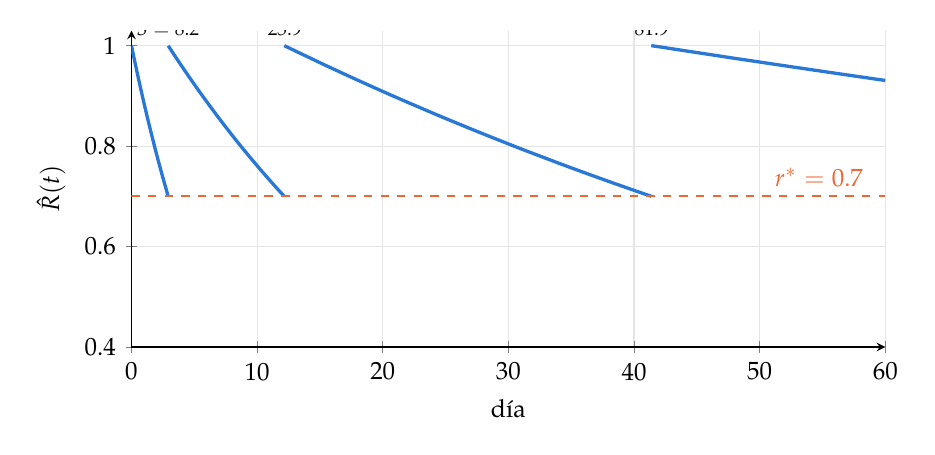
\begin{tikzpicture}
\begin{axis}[
  width=0.92\textwidth, height=5.6cm,
  xlabel={día}, ylabel={$\Rh(t)$}, xmin=0, xmax=60, ymin=0.4, ymax=1.03,
  axis lines=left, grid=major, grid style={gray!20},
  tick label style={font=\small}, label style={font=\small},
]
\addplot[domain=0:2.92, samples=30, very thick, azul] {exp(-x/8.2)};
\addplot[domain=2.92:12.16, samples=40, very thick, azul] {exp(-(x-2.92)/25.9)};
\addplot[domain=12.16:41.37, samples=60, very thick, azul] {exp(-(x-12.16)/81.9)};
\addplot[domain=41.37:60, samples=40, very thick, azul] {exp(-(x-41.37)/258.7)};
\addplot[domain=0:60, dashed, thick, naranja] {0.7};
\node[font=\small, text=naranja, anchor=south east] at (axis cs:59,0.7) {$\rstar=0.7$};
\node[font=\scriptsize, anchor=south] at (axis cs:2.9,1.0) {$\Sh=8.2$};
\node[font=\scriptsize, anchor=south] at (axis cs:12.2,1.0) {$25.9$};
\node[font=\scriptsize, anchor=south] at (axis cs:41.4,1.0) {$81.9$};
\end{axis}
\end{tikzpicture}
\caption{Recuerdo estimado de una habilidad repasada cada vez que $\Rh$ toca $\rstar=0.7$ y se acierta. Cada repaso vuelve a llevar $\Rh$ a 1 y multiplica $\Sh$ por $3.16$, así que las caídas son cada vez más lentas.}
\label{fig:sierra}
\end{figure}

\subsection{El salto del recuerdo}

\begin{equation}
\Rh_k^{+}=\Rh_k+w_{jk}\bigl(1-\Rh_k\bigr),\qquad \Lh_k\leftarrow t+\Sh_k^{+}\,\ln\Rh_k^{+}.
\label{eq:salto}
\end{equation}

\paragraph{Qué calcula.} El recuerdo inmediatamente después de un intento, haya sido acierto o fallo: en ambos casos el estudiante ve la solución. Es la ecuación de salto de \citet{tabibian2019}, $dm=(1-m)\,dN(t)$, ponderada por el peso: el tema principal vuelve a 1 y un prerrequisito recorre una fracción $w$ del camino.

\paragraph{La segunda expresión.} Despeja el instante efectivo $\Lh_k$ que hace que la fórmula~\eqref{eq:memoria}, con la nueva estabilidad $\Sh_k^+$, devuelva exactamente $\Rh_k^+$ en el instante $t$:
\[
\exp\!\Bigl(-\frac{t-\Lh_k}{\Sh_k^+}\Bigr)=\Rh_k^+\iff \Lh_k=t+\Sh_k^+\ln\Rh_k^+.
\]
Si $\Rh_k^+=1$, entonces $\Lh_k=t$. Si $\Rh_k^+<1$, $\Lh_k$ queda en el pasado, como si el repaso completo hubiera ocurrido antes.

\subsection{Asignación de culpa tras un fallo}

Tras un fallo sólo sabemos que $y=0$, no qué componente no se recuperó. Sea $o_k\in\{0,1\}$ el evento (no observado) de recuperar $k$. Por el teorema de Bayes,
\[
b_k=\Pr(o_k=0\mid y=0)=\frac{\Pr(y=0\mid o_k=0)\,\Pr(o_k=0)}{\Pr(y=0)}.
\]
Si $k$ no se recuperó, el problema falla salvo adivinanza: $\Pr(y=0\mid o_k=0)=1-g$. Además $\Pr(o_k=0)=1-\Rh_k^{\,w_{jk}}$ y $\Pr(y=0)=\Pih_j\,s+(1-\Pih_j)(1-g)$. Por lo tanto:

\begin{equation}
b_k=\frac{\bigl(1-\Rh_k^{\,w_{jk}}\bigr)(1-g)}{\Pih_j\,s+\bigl(1-\Pih_j\bigr)(1-g)}.
\label{eq:culpa-completa}
\end{equation}

Con $s=g=0$ se simplifica a la versión que usó la simulación:
\begin{equation}
b_k=\frac{1-\Rh_k^{\,w_{jk}}}{1-\Pih_j}.
\label{eq:culpa}
\end{equation}

\paragraph{Propiedades.}
\begin{itemize}
\item $b_k\in[0,1]$. En~\eqref{eq:culpa} se cumple porque $1-\Rh_k^{w}\le1-\Pih_j$, dado que $\Pih_j\le\Rh_k^{w}$.
\item La culpa es mayor para el componente con menor $\Rh^w$: el sistema culpa a lo que tenía más probabilidad de fallar.
\item Las $b_k$ son probabilidades marginales, así que \emph{pueden sumar más de uno}: es posible que fallen varios componentes a la vez.
\item La versión completa reduce la culpa cuando $\Pih_j\approx1$: un fallo así se explica mejor por descuido que por olvido.
\end{itemize}

\begin{ejemplo}
Un problema de caída libre con $\Rh_{\text{caída}}=0.643$ y $\Rh_{\text{MUA}}=0.793$ ($w=0.5$) da $\Pih=0.643\times0.793^{0.5}=0.573$. Si falla:
\begin{center}\small
\begin{tabular}{@{}lcc@{}}
\toprule
& Culpa simple~\eqref{eq:culpa} & Culpa completa~\eqref{eq:culpa-completa} \\
\midrule
Caída libre & $0.357/0.427=0.84$ & $0.78$ \\
MUA & $0.110/0.427=0.26$ & $0.24$ \\
\bottomrule
\end{tabular}
\end{center}
En cambio, si un problema de un solo componente con $\Rh=0.99$ falla, la culpa simple es 1 (castigo completo), mientras que la completa es $0.0098/(0.99\cdot0.05+0.0098)=0.17$: el sistema lo atribuye sobre todo a un descuido.
\end{ejemplo}

\subsection{Actualización tras un fallo}

\begin{equation}
\Sh_k\leftarrow\max\bigl(\Smin,\ \Sh_k\,(1-\lambda\,b_k)\bigr),\qquad k\in Q(j),\ k\notin D_t,
\label{eq:fallo}
\end{equation}
seguida del salto~\eqref{eq:salto}.

\paragraph{Qué calcula.} Cuánta estabilidad pierde cada componente. Con culpa total ($b_k=1$) pierde una fracción $\lambda$; con culpa parcial, proporcionalmente menos. El piso $\Smin$ evita que la estabilidad llegue a cero.

\paragraph{Por qué también hay salto.} Tras fallar, el estudiante ve la solución resuelta, que funciona como un repaso: el recuerdo inmediato sube aunque la estabilidad baje. El resultado es que el tema vuelve a vencer pronto, que es lo que se quiere después de un fallo.

\subsection{Una sola actualización por habilidad por sesión}

\paragraph{Justificación.} El segundo intento del mismo día ocurre con $\Rh\approx1$. Según~\eqref{eq:acierto} un acierto ahí no aporta ganancia, y un fallo con el tema recién repasado mide más la atención del momento que la memoria de largo plazo. \citet{tabibian2019} tratan del mismo modo cada sesión de Duolingo como un solo repaso. Las habilidades introducidas el mismo día también quedan en $D_t$: su práctica inicial ocurre con el ejemplo resuelto a la vista.

\subsection{Carga de mantenimiento}
\label{sec:admision}

\begin{equation}
\Carga=\sum_{k:\ \iota_k=1}\min\!\left(1,\ \frac{f}{\Sh_k\ln(1/\rstar)}\right).
\label{eq:carga}
\end{equation}

\paragraph{De dónde sale.} Bajo la política, la habilidad $k$ se repasa aproximadamente cada $I_k=\Sh_k\ln(1/\rstar)$ días, así que demanda en promedio $1/I_k$ repasos por día. El factor $f$ convierte días a sesiones ($f=1$ si hay sesión diaria, $f=7/5$ si se estudia cinco días por semana). El $\min(1,\cdot)$ refleja que una habilidad no puede pedir más de un repaso por sesión.

\paragraph{Consecuencia.} Como $\Sh_k$ crece geométricamente con los repasos, la carga de una habilidad madura tiende a cero. El sistema tiene un ritmo natural: al principio admite poco porque todo es frágil, y con el tiempo libera espacio para temas nuevos.

\subsection{Admisión de habilidades nuevas}

\begin{definicion}[Admisibilidad]
Una habilidad $k$ no introducida es admisible en $t$ si
\begin{equation}
\underbrace{\forall p\in\Pre(k):\ \iota_p=1,\ \Sh_p\ge\Slisto,\ \Rh_p(t)\ge\rstar}_{\text{está lista}}
\quad\text{y}\quad
\underbrace{\Carga+m+1\le\rho\,U}_{\text{cabe}},
\label{eq:admision}
\end{equation}
donde $m$ es el número de habilidades ya admitidas ese día. Se admiten hasta $m_{\max}$ por día, en el orden del temario, y cada una ocupa $n_{\mathrm{intro}}$ lugares (un ejemplo resuelto y práctica inicial).
\end{definicion}

\paragraph{La condición ``está lista''.} Es el \emph{outer fringe} de la teoría de espacios de conocimiento \citep{doignon1985}: lo que el estudiante está listo para aprender, con ``consolidado'' en lugar de ``sabido''. El umbral $\Slisto$ controla qué tan firme debe estar la base. Si $\Slisto<\Sh_0$, un tema recién introducido habilita a sus dependientes de inmediato y la compuerta no se nota. Por eso el prototipo usa $\Slisto=12>\Sh_0=8.2$, que exige al menos un repaso exitoso.

\paragraph{La condición ``cabe''.} Convierte la saturación descrita por \citet{reddy2016} en un invariante:
\begin{equation}
\Carga_{\text{después}}\le\rho\,U .
\label{eq:carga-cond}
\end{equation}
Si el modelo de memoria es correcto, la carga esperada nunca excede una fracción $\rho$ del presupuesto diario, y el resto queda disponible para avanzar.

\subsection{Objetivo de la sesión: cobertura submodular}
\label{sec:planificador}

Sean $D=\{k:\ \iota_k=1,\ \Rh_k(t)<\rstar\}$ las habilidades vencidas y $\pi_k=1-\Rh_k(t)$ su prioridad. Esta prioridad tiene la forma de la intensidad óptima de \citet{tabibian2019}, $u^\ast\propto1-m$, convertida en una decisión diaria. Un problema $j$ es \emph{factible} si sus otros componentes cumplen $\Rh_c\ge r_{\min}$; así no se presentan problemas cuyos fallos no diagnosticarían nada. Para un conjunto $A$ de problemas factibles,

\begin{equation}
V(A)=\sum_{k\in D}\pi_k\Bigl[1-\prod_{j\in A}(1-w_{jk})\Bigr].
\label{eq:cobertura}
\end{equation}

\paragraph{Qué calcula.} La ``masa vencida'' que cubre el conjunto de problemas. El corchete es la fracción cubierta de la habilidad $k$: un problema cuyo tema principal es $k$ la cubre entera; dos problemas que la usan como prerrequisito cubren $1-0.5^2=75\%$. El objetivo prefiere un problema integrador que repase varias habilidades vencidas a la vez.

\begin{proposicion}
\label{prop:submod}
$V$ es no negativa, monótona y submodular. Por lo tanto, el algoritmo voraz que agrega en cada paso el problema de mayor ganancia marginal
\begin{equation}
\Delta(j\mid A)=\sum_{k\in D}\pi_k\,\eta_k(A)\,w_{jk},\qquad \eta_k(A)=\prod_{j'\in A}(1-w_{j'k}),
\label{eq:ganancia}
\end{equation}
hasta $U$ problemas, obtiene $V(A_{\mathrm{voraz}})\ge(1-1/e)\max_{|A|\le U}V(A)\approx0.63\max V$.
\end{proposicion}
\begin{proof}
Para cada $k$, $f_k(A)=1-\prod_{j\in A}(1-w_{jk})$ es la probabilidad de que ocurra al menos uno de varios eventos independientes con probabilidades $w_{jk}$. Su ganancia al agregar $j$ es $f_k(A\cup\{j\})-f_k(A)=w_{jk}\,\eta_k(A)\ge0$, que no crece al agrandar $A$ porque $\eta_k$ sólo puede disminuir. Así, $f_k$ es monótona y submodular, y también lo es la combinación no negativa $V=\sum_k\pi_kf_k$. La cota es el resultado clásico de \citet{nemhauser1978}.
\end{proof}

\begin{observacion}
La garantía se refiere a $V$, que es un sustituto de la retención futura; no es una garantía sobre el aprendizaje.
\end{observacion}

El Algoritmo~\ref{alg:sesion} resume la planificación diaria $\Psi$.

\begin{algorithm}[t]
\caption{Planificación de la sesión del día $t$ ($\Psi$)}
\label{alg:sesion}
\small
\begin{algorithmic}[1]
\Require estado $\sigma$, dominio $\Dom$, parámetros $\bm\theta,\bm\varphi$
\State calcular $\Rh_k(t)$ con~\eqref{eq:memoria}; $D\gets\{k:\Rh_k<\rstar\}$; $\pi_k\gets1-\Rh_k$; $\eta_k\gets1$; lugares $\gets U$
\While{lugares $>0$ y existe $j$ factible no elegido con $\Delta(j)>\varepsilon$} \Comment{1. cobertura voraz}
  \State $j^\ast\gets\arg\max_j\Delta(j)$; agregar un problema de $j^\ast$; $\eta_k\gets\eta_k(1-w_{j^\ast k})$; lugares $\gets$ lugares $-1$
\EndWhile
\While{se han admitido menos de $m_{\max}$, lugares $\ge n_{\mathrm{intro}}$ y hay $k$ admisible según~\eqref{eq:admision}} \Comment{2. admisión}
  \State agregar el ejemplo resuelto de $k$ y $n_{\mathrm{intro}}-1$ problemas; lugares $\gets$ lugares $-n_{\mathrm{intro}}$
\EndWhile
\While{lugares $>0$ y queda algún problema factible no elegido} \Comment{3. repaso adelantado}
  \State agregar el de menor $\Rh$
\EndWhile
\Ensure secuencia de actividades $A_t$: repasos, temas nuevos, repasos adelantados
\end{algorithmic}
\end{algorithm}

\subsection{Estimación de parámetros}
\label{sec:estimacion}

Los parámetros $\bm\phi=(\Sh_0,G,\lambda)$ se estiman por máxima verosimilitud con el historial $\Hist$ de un piloto. El modelo es un \emph{filtro determinista}: dados $\bm\phi$ y la secuencia de eventos, el estado antes de cada intento queda determinado (Invariante~\ref{inv:replay}). Entonces la predicción $\hat P_{in}(\bm\phi)$ del intento $n$ del alumno $i$ es una función conocida de $\bm\phi$, y

\begin{equation}
\mathrm{NLL}(\bm\phi)=-\sum_i\sum_n\Bigl[y_{in}\ln\hat P_{in}(\bm\phi)+(1-y_{in})\ln\bigl(1-\hat P_{in}(\bm\phi)\bigr)\Bigr].
\label{eq:nll}
\end{equation}

Para evaluarla se repasa el historial de cada alumno: predecir con~\eqref{eq:observacion}, observar $y$, actualizar con~\eqref{eq:acierto}--\eqref{eq:fallo}. El costo es lineal en el número de intentos. La minimización se hace sin restricciones sobre $(\ln\Sh_0,\ \ln G,\ \operatorname{logit}\lambda)$ con un método sin derivadas como Nelder--Mead.

\paragraph{Identificación.} Cada parámetro queda determinado por un patrón distinto de los datos:
\begin{itemize}
\item $\Sh_0$, por la tasa de acierto en el primer repaso tras distintos intervalos;
\item $G$, por cómo cambia esa tasa después de aciertos espaciados;
\item $\lambda$, por el desempeño después de los fallos.
\end{itemize}
Si el piloto no tiene variación suficiente en los intervalos, los parámetros se confunden (en una de las simulaciones $\hat\lambda$ resultó cercano a cero). Por eso el piloto debe repasar con intervalos variados, no con la política final.

\paragraph{Extensión jerárquica.} Con datos reales conviene un modelo con efecto por alumno y por habilidad, $\ln\Sh_{0,ik}=\mu_k+\alpha_i$, estimado de forma bayesiana. En la arquitectura, eso sólo cambia $\bm\theta$ y $\Theta$.

\subsection{Resumen de parámetros}

\begin{table}[ht]
\centering\small
\caption{Parámetros del sistema. Los del modelo describen a los estudiantes en general; los de la política son decisiones pedagógicas.}
\label{tab:parametros}
\begin{tabularx}{\textwidth}{@{}llllX@{}}
\toprule
& Símbolo & Valor & Origen & Interpretación \\
\midrule
\multirow{7}{*}{\rotatebox{90}{Modelo $\bm\theta$}}
& $\Sh_0$ & 8.2 d & estimado & estabilidad inicial de un tema recién visto \\
& $G$ & 7.2 & estimado & ganancia por acierto \\
& $\lambda$ & 0.13 & estimado & severidad del fallo \\
& $s$ & 0.05 & fijado & descuido \\
& $g$ & 0.02 & fijado & adivinanza \\
& $w_{\mathrm{pre}}$ & 0.5 & fijado & peso de un prerrequisito en un problema \\
& $\Smin$ & 0.2 d & fijado & piso de estabilidad \\
\midrule
\multirow{7}{*}{\rotatebox{90}{Política $\bm\varphi$}}
& $\rstar$ & 0.7 & diseño & retención objetivo: vence si $\Rh<\rstar$ \\
& $r_{\min}$ & 0.6 & diseño & recuerdo mínimo de los componentes de apoyo \\
& $\Slisto$ & 12 d & diseño & firmeza mínima de un prerrequisito \\
& $\rho$ & 0.8 & diseño & fracción máxima para mantenimiento \\
& $U$ & 5--10 & diseño & lugares por sesión \\
& $n_{\mathrm{intro}}$ & 2 & diseño & costo de introducir un tema \\
& $m_{\max}$ & 2--3 & diseño & temas nuevos por día \\
\bottomrule
\end{tabularx}
\end{table}

Los valores estimados provienen del piloto simulado en el grafo de subtemas; con datos reales se reestimarán. La elección de $\rstar$ es una decisión pedagógica: en simulación, valores bajos favorecen la cobertura (más temas vistos) y valores altos la retención por tema.

%=====================================================================
\section{Ejemplo de punta a punta}
\label{sec:ejemplo}
%=====================================================================

Seguimos a un estudiante en el subgrafo MRU $\to$ MUA $\to$ Caída libre, con $U=3$, $\Sh_0=6.8$, $G=6.18$, $\lambda=0.19$ y $\Slisto=7$. El alumno simulado aprende y olvida con reglas que el sistema no conoce; el sistema sólo ve aciertos y fallos.

\begin{enumerate}
\item \textbf{Día 0.} No hay nada introducido; MRU no tiene prerrequisitos y la carga es 0, así que se admite (\eqref{eq:admision}). El sistema fija $\Sh_{\text{MRU}}=6.8$ y $\Lh=0$. Los dos problemas de práctica no actualizan nada ($\text{MRU}\in D_0$).
\item \textbf{Día 1.} $\Rh_{\text{MRU}}=e^{-1/6.8}=0.863$: no vence. MUA no es admisible porque $\Sh_{\text{MRU}}=6.8<7$. Los lugares se llenan con repasos adelantados de MRU. Tras un acierto,~\eqref{eq:acierto} da $\Sh_{\text{MRU}}=6.8\,[1+6.18(1-0.863)]=12.55$.
\item \textbf{Día 2.} Ahora $\Sh_{\text{MRU}}=12.55\ge7$, $\Rh_{\text{MRU}}=0.923\ge0.7$ y la carga es $1/(12.55\ln(1/0.7))=0.22$ (con $f=1$), así que $0.22+1\le2.4$ y MUA entra. Un problema de MUA repasa MRU con $w=0.5$: $\Sh_{\text{MRU}}=12.55\,[1+0.5\cdot6.18\cdot0.077]=15.52$ y, por~\eqref{eq:salto}, $\Rh_{\text{MRU}}=0.923+0.5(1-0.923)=0.962$.
\item \textbf{Día 4.} Entra caída libre.
\item \textbf{Día 7}, tras el fin de semana. Caída libre es la única vencida ($\Rh=0.643$). Por~\eqref{eq:ganancia}, el problema de caída libre tiene ganancia $0.357$ y se elige. El estudiante falla. Con~\eqref{eq:culpa}, $b_{\text{caída}}=0.84$ y $b_{\text{MUA}}=0.26$; con~\eqref{eq:fallo}, $\Sh_{\text{caída}}$ pasa de $6.80$ a $5.72$ y $\Sh_{\text{MUA}}$ de $15.52$ a $14.76$. El sistema atribuyó el fallo a caída libre sin ver qué pasó en la cabeza del estudiante.
\end{enumerate}

%=====================================================================
\section{Evidencia de simulación}
\label{sec:evidencia}
%=====================================================================

El primer documento del proyecto evalúa el modelo con un simulador Monte Carlo. Allí, el alumno ``verdadero'' está deliberadamente mal especificado respecto al modelo: olvido de ley de potencia, ganancia tipo FSRS y recuperación oculta por componente. Sobre el grafo de 168 subtemas, con 300 alumnos por política y la probabilidad de resolver un problema nuevo 30 días después del curso como métrica:

\begin{itemize}
\item el sistema supera a Anki SM-2 por $+0.090$ y $+0.047$ (según el supuesto sobre bases débiles), sobre todo porque introduce más temas (106 frente a 71); Anki deja más subtemas dominados;
\item espaciar los repasos mejora la métrica en $+0.20$ frente a la enseñanza bloqueada;
\item si el grafo tiene dependencias falsas (cadenas lineales), la ventaja desaparece o se invierte.
\end{itemize}

\begin{figure}[t]
\centering
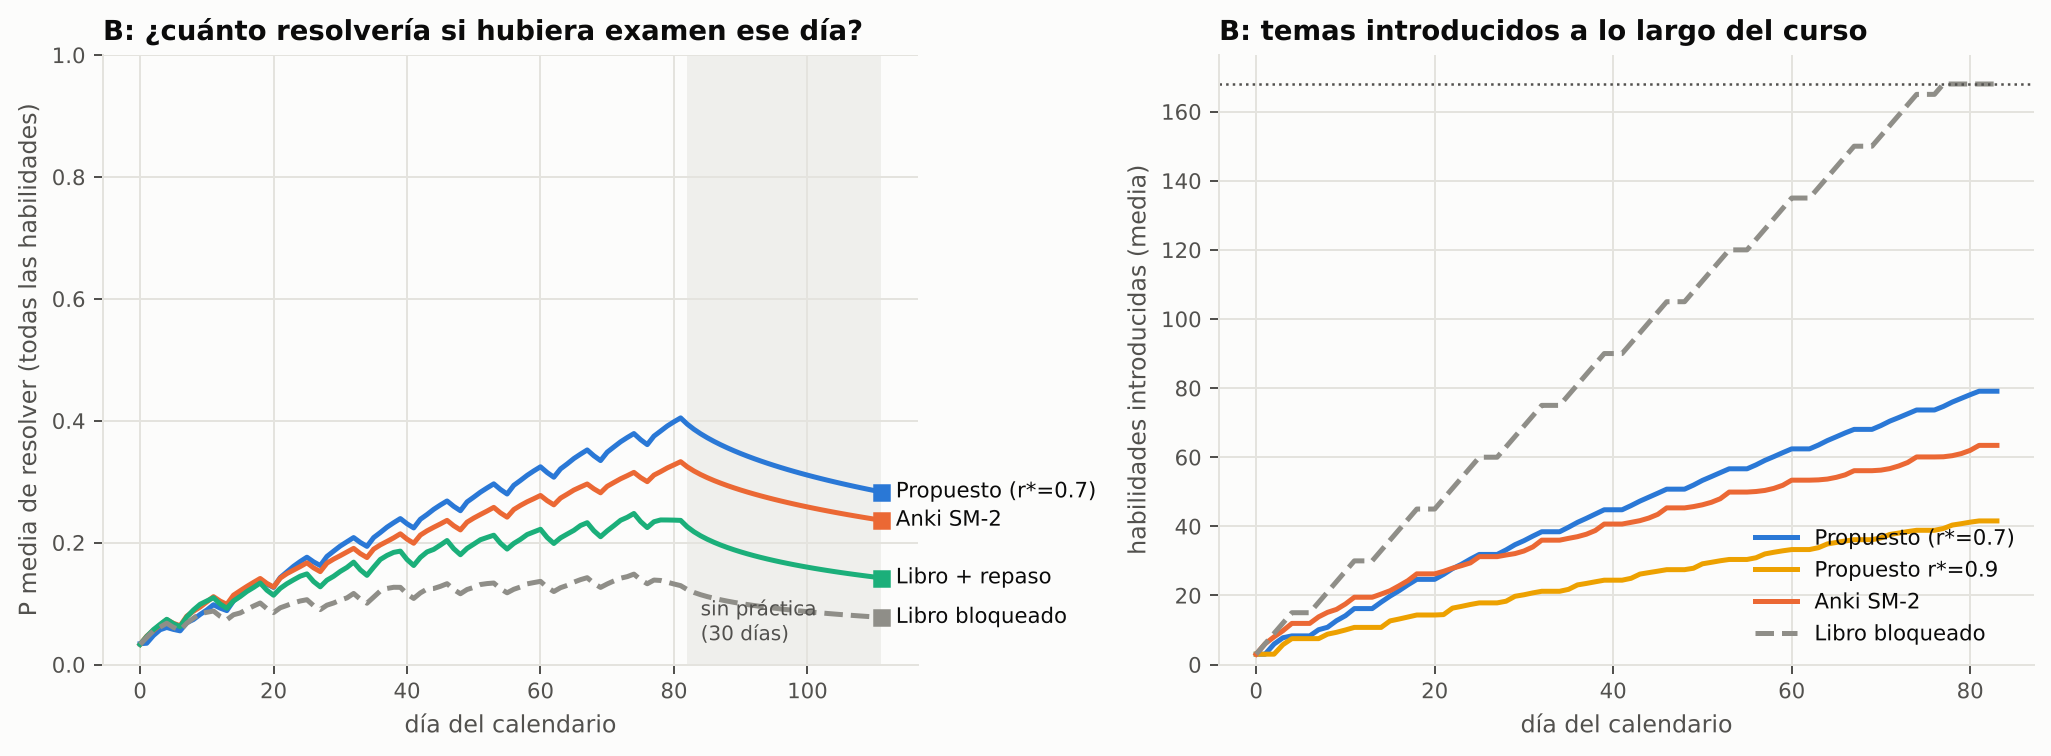
\includegraphics[width=\textwidth]{figuras/subtemas_trayectorias.png}
\caption{Simulación sobre el grafo de 168 subtemas. Izquierda: probabilidad media de resolver si el examen fuera ese día; la zona gris son 30 días sin práctica. Derecha: temas introducidos. Anki se atasca con sus repasos vencidos; con $\rstar=0.9$ el sistema repasa tan seguido que casi no avanza.}
\label{fig:sim}
\end{figure}

%=====================================================================
\section{El prototipo como instancia de la arquitectura}
\label{sec:prototipo}
%=====================================================================

El prototipo es una aplicación web con dos paneles: lo que ve el estudiante y lo que hace el sistema. Un botón adelanta el reloj un día. Es \emph{una} instancia de la arquitectura; la Tabla~\ref{tab:mapeo} muestra la correspondencia.

\begin{table}[ht]
\centering\small
\caption{Correspondencia entre los componentes abstractos y el prototipo.}
\label{tab:mapeo}
\begin{tabularx}{\textwidth}{@{}lX@{}}
\toprule
Componente & En el prototipo \\
\midrule
Dominio $\Dom$ & dos archivos de datos: el grafo de 13 habilidades y 33 plantillas paramétricas \\
Generación $\Gamma$ & sorteo de variables y evaluación de fórmulas de cada plantilla \\
Estado $\sigma$ y recuerdo $\Rh$ & tabla de $(\Sh_k,\Lh_k)$ con $\Rh$ calculado al momento \\
Predicción y actualización $\Phi$ & función que predice $\hat P$, registra el resultado y aplica~\eqref{eq:acierto}--\eqref{eq:fallo} \\
Planificación $\Psi$ & Algoritmo~\ref{alg:sesion}, ejecutado al pasar el día \\
Historial $\Hist$ & bitácora de eventos visible en el panel del sistema \\
Calibración $\Theta$ & no incluida: los parámetros vienen de la simulación y se pueden editar a mano \\
\bottomrule
\end{tabularx}
\end{table}

Una diferencia con la arquitectura: el prototipo guarda el estado y la bitácora por separado, en lugar de reconstruir el estado a partir de la bitácora. Para cumplir el Invariante~\ref{inv:replay} hay que registrar en la bitácora cada instancia presentada y cada cambio de parámetros, y derivar el estado de ella.

%=====================================================================
\section{Limitaciones y trabajo futuro}
%=====================================================================

\begin{enumerate}
\item \textbf{Alcance.} Sólo física clásica de preparatoria. La extensión a matemáticas requiere un grafo y un banco nuevos, no un modelo nuevo.
\item \textbf{Grafo.} Las dependencias entre subtemas son un borrador sin validación docente, y la figura y la lista formal deben reconciliarse.
\item \textbf{Parámetros.} Los valores de $\Sh_0$, $G$ y $\lambda$ provienen de un piloto simulado. Un piloto real con intervalos variados es el siguiente paso.
\item \textbf{Supuestos del modelo}: olvido exponencial, independencia entre componentes, $w_{\mathrm{pre}}$ común y estabilidad inicial común. Todos se pueden contrastar con los datos del piloto.
\item \textbf{Fenómenos no modelados}: intercalado \citep{rohrer2015}, fatiga, motivación y aprendizaje con ejemplos resueltos.
\item \textbf{Validación en aula}: un diseño intra-sujeto contrabalanceado \citep{lindsey2014}, con prueba diferida a 30 días.
\end{enumerate}

%=====================================================================
\appendix
\section{Aristas del grafo de unidades}
\label{app:aristas}
%=====================================================================

La especificación formal usada por el simulador tiene 26 aristas entre las 15 unidades (origen $\to$ destino):

\begin{center}\small
\setlength{\tabcolsep}{4pt}\begin{tabular}{@{}ll@{\hspace{1.2em}}ll@{}}
\toprule
Origen & Destino & Origen & Destino \\
\midrule
Magnitudes y unidades & Vectores & Leyes de Newton & Cantidad de movimiento \\
Vectores & MRU & Leyes de Newton & Trabajo y energía \\
Vectores & MUA & Aplicaciones de Newton & Trabajo y energía \\
Vectores & Movimiento en el plano & Trabajo y energía & Potencia \\
MRU & MUA & Cantidad de movimiento & Impulso y colisiones \\
MUA & Tiro parabólico & Trabajo y energía & Energía mecánica \\
Movimiento en el plano & Tiro parabólico & Cantidad de movimiento & Sistemas de partículas \\
Vectores & Leyes de Newton & Leyes de Newton & Sistemas de partículas \\
MUA & Leyes de Newton & Impulso y colisiones & Sistemas de partículas \\
Movimiento en el plano & Aplicaciones de Newton & Vectores & Rotación \\
Tiro parabólico & Aplicaciones de Newton & Aplicaciones de Newton & Rotación \\
Leyes de Newton & Aplicaciones de Newton & Trabajo y energía & Rotación \\
 & & Energía mecánica & Rotación \\
 & & Sistemas de partículas & Rotación \\
\bottomrule
\end{tabular}
\end{center}

%=====================================================================
\section{Subgrafo del prototipo}
\label{app:prototipo}
%=====================================================================

\begin{center}\small
\begin{tabular}{@{}lll@{}}
\toprule
Código & Habilidad & Prerrequisitos \\
\midrule
MAG3 & Conversión de unidades & --- \\
VEC3 & Componentes cartesianas & --- \\
VEC10 & Descomposición de vectores & VEC3 \\
MRU6 & Velocidad constante & MAG3 \\
MRU7 & Ecuación de posición & MRU6 \\
MUA4 & Ecuaciones del movimiento acelerado & MRU7 \\
MUA7 & Relación entre velocidad y desplazamiento & MUA4 \\
MUA11 & Caída libre & MUA4 \\
MUA12 & Lanzamiento vertical & MUA11, MUA7 \\
TIR2 & Descomposición de la velocidad inicial & VEC10 \\
TIR7 & Tiempo de vuelo & TIR2, MUA12 \\
TIR8 & Altura máxima & TIR2, MUA12 \\
TIR9 & Alcance horizontal & TIR7, MRU7 \\
\bottomrule
\end{tabular}
\end{center}

\begin{thebibliography}{99}
\small

\bibitem[{Arthur et~al.(1998)}]{arthur1998}
Arthur, W., Bennett, W., Stanush, P.~L. y McNelly, T.~L. (1998).
\newblock Factors that influence skill decay and retention: A quantitative review and analysis.
\newblock \emph{Human Performance}, 11(1):57--101.

\bibitem[{Barzagar~Nazari y Ebersbach(2019)}]{barzagar2019}
Barzagar~Nazari, K. y Ebersbach, M. (2019).
\newblock Distributing mathematical practice of third and seventh graders: Applicability of the spacing effect in the classroom.
\newblock \emph{Applied Cognitive Psychology}, 33(2):288--298.

\bibitem[{Cen et~al.(2006)}]{cen2006}
Cen, H., Koedinger, K. y Junker, B. (2006).
\newblock Learning factors analysis: A general method for cognitive model evaluation and improvement.
\newblock En \emph{Intelligent Tutoring Systems (ITS 2006)}, pp.~164--175. Springer.

\bibitem[{Cepeda et~al.(2006)}]{cepeda2006}
Cepeda, N.~J., Pashler, H., Vul, E., Wixted, J.~T. y Rohrer, D. (2006).
\newblock Distributed practice in verbal recall tasks: A review and quantitative synthesis.
\newblock \emph{Psychological Bulletin}, 132(3):354--380.

\bibitem[{Cepeda et~al.(2008)}]{cepeda2008}
Cepeda, N.~J., Vul, E., Rohrer, D., Wixted, J.~T. y Pashler, H. (2008).
\newblock Spacing effects in learning: A temporal ridgeline of optimal retention.
\newblock \emph{Psychological Science}, 19(11):1095--1102.

\bibitem[{Choffin et~al.(2019)}]{choffin2019}
Choffin, B., Popineau, F., Bourda, Y. y Vie, J.-J. (2019).
\newblock DAS3H: Modeling student learning and forgetting for optimally scheduling distributed practice of skills.
\newblock En \emph{Proceedings of the 12th International Conference on Educational Data Mining (EDM 2019)}. arXiv:1905.06873.

\bibitem[{Choffin et~al.(2021)}]{choffin2021}
Choffin, B., Popineau, F. y Bourda, Y. (2021).
\newblock Extending adaptive spacing heuristics to multi-skill items.
\newblock \emph{Journal of Educational Data Mining}, 13(3).

\bibitem[{Corbett y Anderson(1994)}]{corbett1994}
Corbett, A.~T. y Anderson, J.~R. (1994).
\newblock Knowledge tracing: Modeling the acquisition of procedural knowledge.
\newblock \emph{User Modeling and User-Adapted Interaction}, 4(4):253--278.

\bibitem[{de~la Torre(2011)}]{delatorre2011}
de~la Torre, J. (2011).
\newblock The generalized DINA model framework.
\newblock \emph{Psychometrika}, 76(2):179--199.

\bibitem[{Doignon y Falmagne(1985)}]{doignon1985}
Doignon, J.-P. y Falmagne, J.-C. (1985).
\newblock Spaces for the assessment of knowledge.
\newblock \emph{International Journal of Man-Machine Studies}, 23(2):175--196.

\bibitem[{Hunziker et~al.(2019)}]{hunziker2019}
Hunziker, A., Chen, Y., Mac~Aodha, O., Gomez-Rodriguez, M., Krause, A., Perona, P., Yue, Y. y Singla, A. (2019).
\newblock Teaching multiple concepts to a forgetful learner.
\newblock En \emph{Advances in Neural Information Processing Systems 32 (NeurIPS 2019)}.

\bibitem[{Junker y Sijtsma(2001)}]{junker2001}
Junker, B.~W. y Sijtsma, K. (2001).
\newblock Cognitive assessment models with few assumptions, and connections with nonparametric item response theory.
\newblock \emph{Applied Psychological Measurement}, 25(3):258--272.

\bibitem[{Koedinger et~al.(2012)}]{koedinger2012}
Koedinger, K.~R., Corbett, A.~T. y Perfetti, C. (2012).
\newblock The Knowledge-Learning-Instruction framework: Bridging the science-practice chasm to enhance robust student learning.
\newblock \emph{Cognitive Science}, 36(5):757--798.

\bibitem[{Lindsey et~al.(2014)}]{lindsey2014}
Lindsey, R.~V., Shroyer, J.~D., Pashler, H. y Mozer, M.~C. (2014).
\newblock Improving students' long-term knowledge retention through personalized review.
\newblock \emph{Psychological Science}, 25(3):639--647.

\bibitem[{Nemhauser et~al.(1978)}]{nemhauser1978}
Nemhauser, G.~L., Wolsey, L.~A. y Fisher, M.~L. (1978).
\newblock An analysis of approximations for maximizing submodular set functions---I.
\newblock \emph{Mathematical Programming}, 14(1):265--294.

\bibitem[{Pavlik et~al.(2009)}]{pavlik2009}
Pavlik, P.~I., Cen, H. y Koedinger, K.~R. (2009).
\newblock Performance factors analysis: A new alternative to knowledge tracing.
\newblock En \emph{Artificial Intelligence in Education (AIED 2009)}, pp.~531--538. IOS Press.

\bibitem[{Pyc y Rawson(2009)}]{pyc2009}
Pyc, M.~A. y Rawson, K.~A. (2009).
\newblock Testing the retrieval effort hypothesis: Does greater difficulty correctly recalling information lead to higher levels of memory?
\newblock \emph{Journal of Memory and Language}, 60(4):437--447.

\bibitem[{Reddy et~al.(2016)}]{reddy2016}
Reddy, S., Labutov, I., Banerjee, S. y Joachims, T. (2016).
\newblock Unbounded human learning: Optimal scheduling for spaced repetition.
\newblock En \emph{Proceedings of the 22nd ACM SIGKDD International Conference on Knowledge Discovery and Data Mining}, pp.~1815--1824.

\bibitem[{Rohrer et~al.(2015)}]{rohrer2015}
Rohrer, D., Dedrick, R.~F. y Stershic, S. (2015).
\newblock Interleaved practice improves mathematics learning.
\newblock \emph{Journal of Educational Psychology}, 107(3):900--908.

\bibitem[{Rohrer y Taylor(2007)}]{rohrer2007}
Rohrer, D. y Taylor, K. (2007).
\newblock The shuffling of mathematics problems improves learning.
\newblock \emph{Instructional Science}, 35(6):481--498.

\bibitem[{Settles y Meeder(2016)}]{settles2016}
Settles, B. y Meeder, B. (2016).
\newblock A trainable spaced repetition model for language learning.
\newblock En \emph{Proceedings of the 54th Annual Meeting of the Association for Computational Linguistics (ACL 2016)}, pp.~1848--1858.

\bibitem[{Skycak(2023)}]{skycak2023}
Skycak, J. (2023).
\newblock Individualized spaced repetition in hierarchical knowledge structures.
\newblock \url{https://www.justinmath.com/individualized-spaced-repetition-in-hierarchical-knowledge-structures/}.

\bibitem[{Su et~al.(2023)}]{su2023}
Su, J., Ye, J., Nie, L., Cao, Y. y Chen, Y. (2023).
\newblock Optimizing spaced repetition schedule by capturing the dynamics of memory.
\newblock \emph{IEEE Transactions on Knowledge and Data Engineering}, 35(10):10085--10097.

\bibitem[{Tabibian et~al.(2019)}]{tabibian2019}
Tabibian, B., Upadhyay, U., De, A., Zarezade, A., Schölkopf, B. y Gomez-Rodriguez, M. (2019).
\newblock Enhancing human learning via spaced repetition optimization.
\newblock \emph{Proceedings of the National Academy of Sciences}, 116(10):3988--3993.

\bibitem[{Tatsuoka(1983)}]{tatsuoka1983}
Tatsuoka, K.~K. (1983).
\newblock Rule space: An approach for dealing with misconceptions based on item response theory.
\newblock \emph{Journal of Educational Measurement}, 20(4):345--354.

\bibitem[{Upadhyay et~al.(2021)}]{upadhyay2021}
Upadhyay, U., Lancashire, G., Moser, C. y Gomez-Rodriguez, M. (2021).
\newblock Large-scale randomized experiments reveals that machine learning-based instruction helps people memorize more effectively.
\newblock \emph{npj Science of Learning}, 6:26.

\bibitem[{Woźniak(1990)}]{wozniak1990}
Woźniak, P.~A. (1990).
\newblock \emph{Optimization of learning}.
\newblock Tesis de maestría, Universidad Tecnológica de Poznań.

\bibitem[{Ye et~al.(2022)}]{ye2022}
Ye, J., Su, J. y Cao, Y. (2022).
\newblock A stochastic shortest path algorithm for optimizing spaced repetition scheduling.
\newblock En \emph{Proceedings of the 28th ACM SIGKDD Conference on Knowledge Discovery and Data Mining}, pp.~4381--4390.

\end{thebibliography}


\end{document}
